% This is a basic template for H. Shim

\documentclass[t, 10pt, handout]{beamer}
\setbeameroption{hide notes}
  
\def\mynote{aa}   % Comment if mynote wants to appear

\mode<presentation>
{
  \usetheme{boxes}
  \usefonttheme[onlymath]{serif}
  \setbeamercovered{transparent}
}

\setbeamertemplate{navigation symbols}{}
% removes the navigation symbols
\setbeamertemplate{footline}[frame number]
%\setbeamertemplate{footline}[text line]{%
%color setting more or less matching U of A colors
%\setbeamercolor*{palette secondary}{use=structure,fg=white,bg=structure.fg!55!black}
%\setbeamercolor*{palette tertiary}{use=structure,fg=white,bg=red!50!black}

\usepackage{kotex}
\usepackage[english]{babel}
\usepackage[T1]{fontenc}
\usepackage{comment}
\usepackage{mathtools}
\usepackage{setspace}

\colorlet{Darkred}{red!50!black}
\colorlet{Darkgreen}{green!50!black}
\colorlet{Darkblue}{blue!70!black}
\newcommand{\colb}{\color{Darkblue}}
\newcommand{\colgr}{\color{gray}}
\newcommand{\colg}{\color{Darkgreen}}
\newcommand{\colr}{\color{Darkred}}

% Define Environment:
\newtheorem{thm}{\bf Theorem}
\newtheorem{prop}{\bf Proposition}
\newtheorem{lem}{\bf Lemma}
\newtheorem{assmpt}{\bf Assumption}
\newtheorem{defn}{\bf Definition}
\newtheorem{exmp}{\bf Example}
\newtheorem{cor}{\bf Corollary}
\newtheorem{condi}{\bf Condition}
%=== Non-italic Theorem Environment by Vin
\newtheorem{rem1}{\bf Remark}
\newenvironment{rem}{\begin{rem1}\normalfont}{\end{rem1}}
%=== New Example Environment by Vin
\newcounter{Examp}
\newenvironment{exam}{\stepcounter{Examp} \medskip \noindent {\bf Example \arabic{Examp}.}}{ \medskip }

%=== New Example Environment by Vin
\newcounter{exer}
\newenvironment{exer}{\stepcounter{exer} \medskip \noindent {\bf Exercise \arabic{exer}.}}{ \medskip }


% Define Some Notation:

\newcommand{\nn}{{\mathfrak{n}}}

\newcommand{\R}{\ensuremath{{\mathbb R}}}
\newcommand{\Z}{\ensuremath{{\mathbb Z}}}
\newcommand{\N}{\ensuremath{{\mathbb N}}}

\newcommand{\AAA}{{\mathcal A}}
\newcommand{\CC}{{\mathcal C}}
\newcommand{\DD}{{\mathcal D}}
\newcommand{\EE}{{\mathcal E}}
\newcommand{\FF}{{\mathcal F}}
\newcommand{\KK}{{\mathcal K}}
\newcommand{\LL}{{\mathcal L}}
\newcommand{\MM}{{\mathcal M}}
\newcommand{\NN}{{\mathcal N}}
\newcommand{\OO}{{\mathcal O}}
\newcommand{\PP}{{\mathcal P}}
\newcommand{\QQ}{{\mathcal Q}}
\newcommand{\RR}{{\mathcal R}}
\newcommand{\SSS}{{\mathcal S}}
\newcommand{\TT}{{\mathcal T}}
\newcommand{\UU}{{\mathcal U}}
\newcommand{\VV}{{\mathcal V}}
\newcommand{\WW}{{\mathcal W}}
\newcommand{\XX}{{\mathcal X}}
\newcommand{\YY}{{\mathcal Y}}
\newcommand{\cN}{\ensuremath{\mathcal{N}}}

\newcommand{\KL}{{\mathcal{KL}}}
\newcommand{\sat}{\ensuremath{{\rm sat}}}

\newcommand{\triend}{\hfill \ensuremath{\lhd}}
\DeclareMathOperator{\rank}{rank}

\newcommand{\cvector}[1]{\left(\!\!\!\begin{array}{c} #1 \end{array}\!\!\!\right)}
\newcommand{\setdef}[2]{\left\{\ #1\ \left|\ #2\ \right.\right\}}

\setbeamertemplate{itemize subitem}[circle]

\setstretch{1.1}

\setbeamersize{text margin left=0.5cm}  % <- like this
\setbeamersize{text margin right=0.5cm} % <- like this


%%%%%%%%%%% Contents %%%%%%%%%

\title{[ECDL3-Unit3]
Series RLC Band-pass Filter \\ 
and Parallel RLC Band-rejection Filter}

\author{Sewon Kim}
\vspace{-0.5cm}
\institute{\normalsize Department of Electrical and Computer Engineering \\
University of Seoul
	\vspace{1cm}
\\
\vspace{-0.2cm}}

\date{2024.03.21}




\begin{document}


\begin{frame}[plain]
  \titlepage
\end{frame}


\begin{frame}{Contents}
    \begin{itemize}
        \item[$\bullet$] {\large Series RLC Band-pass Filter}
        \vspace{5pt}
        \begin{itemize}
            \item[$\bullet$] {\normalsize Series RLC circuit}
            \vspace{5pt}
            \item[$\bullet$] {\normalsize Frequency response of admittance $I/V_s$ (RL = 1T Ohm)}
            \vspace{5pt}
            \item[$\bullet$] {\normalsize Frequency response of voltage gain $V_0/V_s$ (RL = 1T Ohm)}
            \vspace{5pt}
            \item[$\bullet$] {\normalsize Frequency response of voltage gain $V_0/V_s$ (RL = 1T Ohm or 50 Ohm)}
            \vspace{5pt}
            \item[$\bullet$] {\normalsize Analysis table}
        \end{itemize}
        \vspace{10pt}
        \item[$\bullet$] {\large Parallel RLC Band-rejection Filter}
        \vspace{5pt}
        \begin{itemize}
            \item[$\bullet$] {\normalsize Parallel RLC circuit}
            \vspace{5pt}
            \item[$\bullet$] {\normalsize Frequency response of impedance $V_s/I$ (RL = 0)}
            \vspace{5pt}
            \item[$\bullet$] {\normalsize Frequency response of voltage gain $V_0/V_s$ (RL = 50 Ohm or 2K Ohm)}
            \vspace{5pt}
            \item[$\bullet$] {\normalsize Analysis table}
        \end{itemize}
    \end{itemize}
\end{frame}









\begin{frame}{Series RLC Band-pass Filter (a)}
    \begin{figure}
        \centering
        \includegraphics[width=0.7\textwidth,height=0.7\textheight,keepaspectratio]{img/lab1-d-circuit.png}
	\begin{itemize}
		\item $Q = 0.4, \; f_0 = 5000/\pi (= 1591.55)$ Hz   (RL = $\infty$)
		\item $Q = \dfrac{1}{R}\sqrt{\dfrac{L}{C}}, \; w_0 := \dfrac{1}{\sqrt{LC}} \rightarrow \mathbf{R = 250\Omega, \; C = 1\mu F}$ (series RLC circuit)
	\end{itemize}
    \end{figure}
\end{frame}


\begin{frame}{Series RLC Band-pass Filter (b)}
    \begin{figure}
        \centering
        \includegraphics[width=0.6\textwidth,height=0.6\textheight,keepaspectratio]{img/lab1-b-graph.png}
	\begin{itemize}
		\item $20\log (10^{-47.96/20}/\sqrt{2}) = -50.97$ dB
	\end{itemize}
    \end{figure}
\end{frame}

\begin{frame}{Series RLC Band-pass Filter (c)}
    \begin{figure}
        \centering
        \includegraphics[width=0.6\textwidth,height=0.6\textheight,keepaspectratio]{img/lab1-c-graph.png}
	\begin{itemize}
            \item $I/V_s$ and $V_o/V_s$ have the same resonance frequency and the same cutoff frequencies.
            \item $I/V_s$ and $V_o/V_s$ have consistent phase shifts with frequency.
            \item $20\log (1/\sqrt{2}) = -3.01$ dB
	\end{itemize}
    \end{figure}
\end{frame}

\begin{frame}{Series RLC Band-pass Filter (d)}
    \begin{figure}
        \centering
        \includegraphics[width=0.6\textwidth,height=0.6\textheight,keepaspectratio]{img/lab1-d-graph.png}
	\begin{itemize}
		\item As the load resistance RL increases, the bandwidth increases.
	\end{itemize}
    \end{figure}
\end{frame}

\begin{frame}{Series RLC Band-pass Filter (e)}
    \begin{figure}
        \centering
        \includegraphics[width=0.7\textwidth,height=0.7\textheight,keepaspectratio]{img/lab1-e-table.png}
	\begin{itemize}
		\item As the load resistance RL increases, the quality factor decreases.
            \\ $R_{eq} = \dfrac{R \cdot R_L}{R + R_L} = R - \dfrac{R^2}{R + R_L}$, $Q = \dfrac{1}{R_{eq}}\sqrt{\dfrac{L}{C}}$ (series RLC circuit)
	\end{itemize}
	\begin{itemize}
		\item The simulated resonant frequency (1592.21 Hz) matches the theoretical resonant frequency (1591.55 Hz) within 0.04\%.
		\item That simulated quality factor (0.4) matches correctly with the theoretical quality factor (0.4) when RL = INF(1TOhm).
	\end{itemize}    
        \begin{itemize}
            \item $Q := \dfrac{\text{(Central frequency)}}{\text{(Bandwidth)}} = \dfrac{\sqrt{\omega_{LO}\omega_{HI}}}{\omega_{HI}-\omega_{LO}}$
        \end{itemize}
    \end{figure}
\end{frame}







\begin{frame}{Parallel RLC Band-rejection Filter (a)}
    \begin{figure}
        \centering
        \includegraphics[width=0.7\textwidth,height=0.7\textheight,keepaspectratio]{img/lab2-c-circuit.png}
        \begin{itemize}
		\item Quality factor $Q = R\sqrt{\dfrac{C}{L}} = 2.5$ (Parallel RLC circuit)
            \item Resonance frequency $f_0 = \dfrac{1}{2\pi\sqrt{LC}} = 1591.55$ Hz (RL = 0)
	\end{itemize}
    \end{figure}
\end{frame}

\begin{frame}{Parallel RLC Band-rejection Filter (b)}
    \begin{figure}
        \centering
        \includegraphics[width=0.6\textwidth,height=0.6\textheight,keepaspectratio]{img/lab2-b-graph.png}
	\begin{itemize}
            \item The simulated resonant frequency (1592.21 Hz) matches the theoretical resonant frequency (1591.55 Hz) within 0.04\% when RL = 0
		\item That simulated quality factor (2.51) matches correctly with the theoretical quality factor (2.5) when RL = 0.
	\end{itemize}   
    \end{figure}
\end{frame}

\begin{frame}{Series RLC Band-rejection Filter (c)}
	\begin{columns}
		\column[t]{0.5\textwidth}
  
		\begin{figure}
		{\includegraphics[width=1.0\columnwidth]{img/lab2-c-graph.png}}
		\end{figure}

		\column[t]{0.5\textwidth}

  		\begin{figure}
		{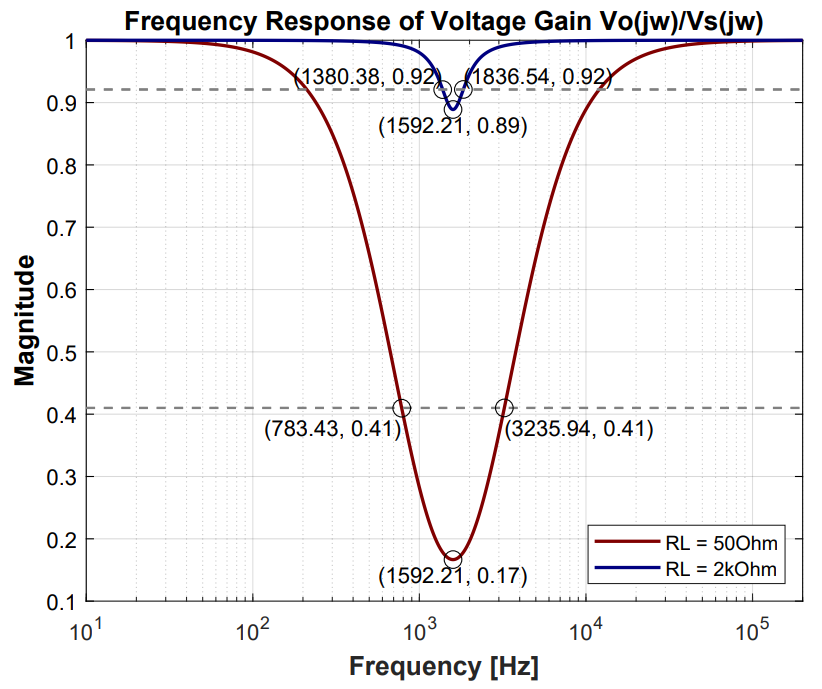
\includegraphics[width=1.0\columnwidth]{img/lab2-d-graph.png}}
		\end{figure}
	\end{columns}
	\begin{itemize}
            \item As the load resistance RL increases, the bandwidth decreases \\
            and the minimum value increases.
            \item $V_s/I$ and $V_o/V_s$ have the same resonance frequency regardless of RL \\
            and different phase shifts with frequency.
    	\item $1-(1-0.17)/\sqrt{2} = 0.41$, $1-(1-0.89)/\sqrt{2} = 0.92$
    \end{itemize}   
\end{frame}	

\begin{frame}{Parallel RLC Band-rejection Filter (d)}
    \begin{figure}
        \centering
        \includegraphics[width=0.7\textwidth,height=0.7\textheight,keepaspectratio]{img/lab2-d-table.png}
        \begin{itemize}
            \item As the load resistance RL increases, the quality factor increases.
        \end{itemize}
	\begin{itemize}
		\item The simulated resonant frequency (1592.21 Hz) matches the theoretical resonant frequency (1591.55 Hz) within 0.04\% regardless of RL
	\end{itemize}   
    \end{figure}
\end{frame}

\end{document}

\section{}